
\documentclass[sigconf]{acmart}

\AtBeginDocument{%
  \providecommand\BibTeX{{%
    \normalfont B\kern-0.5em{\scshape i\kern-0.25em b}\kern-0.8em\TeX}}}


\setcopyright{acmcopyright}
\copyrightyear{2022}
\acmYear{2022}
\acmDOI{XXXXXXX.XXXXXXX}

\acmConference[CCS'XX]{Computer and Communications Security}{Month dates,
  Year}{Venue}

\acmPrice{15.00}
\acmISBN{978-1-4503-XXXX-X/22/11}

\usepackage{xcolor}
\usepackage{listings}
 \lstset{language=Caml}
  \lstset{tabsize=2}
  \lstset{escapeinside={@}{@}}
  
\usepackage{ dsfont }  
\usepackage{algorithmicx}
\usepackage{algorithm,float}
\usepackage{algpseudocode}
\usepackage{paralist}
\usepackage{listings}% http://ctan.org/pkg/listings
\usepackage{xcolor}

\newcommand{\yannis}[1]{\textcolor{blue}{Yannis: #1}}
\newcommand{\todo}[1]{\textcolor{red}{todo: #1}}
\newcommand{\priyanka}[1]{\textcolor{purple}{priyanka: #1}}
\newcommand{\pair}[2]{{\langle \ensuremath{#1, #2} \rangle}}
\newcommand{\DB}[1]{\mathcal{D}(#1)}
\newcommand{\kw}[1]{\mathcal{K}(#1)}
\newcommand{\vol}[1]{\lvert{#1}\rvert}
\newcommand{\ceil}[1]{\lceil #1 \rceil}
\newcommand{\Orion}{\textsc{Orion }}
\newcommand{\BigOrion}{\textsc{BigOrion }}
\newcommand{\Bigorion}{\textsc{BigOrion}}
\newcommand{\Mitra}{\textsc{Mitra }}
\newcommand{\Mitrap}{\textsc{Mitra}$^{+}$ }
\newcommand{\Orionsq}{\textsc{Orion}$^{2}$ }
\newcommand{\Orionp}{\textsc{Orion}$^{+}$ }
\newcommand{\al}{\alpha}
\newcommand{\In}[1]{\ensuremath{\mathcal{I}(#1)}}
\newcommand{\tred}[1]{\textcolor{red}{#1}}
\newcommand{\tblue}[1]{\textcolor{blue}{#1}}
\newcommand{\tpurp}[1]{\textcolor{purple}{#1}}
\newcommand{\tvol}[1]{\textsf{tvol}({#1})}
\newcommand{\tvold}[1]{\textsf{tvol}'({#1})}
\newcommand{\tvoldx}[1]{\textsf{tvol}_{x}'({#1})}
\newcommand{\idvol}[1]{\textsf{idvol}({#1})}
\newcommand{\tvolx}[1]{\textsf{tvol}_{x}({#1})}

\lstset{emph={%
    return, fetch%
    },emphstyle={\color{magenta}}%
}
\definecolor{codegreen}{rgb}{0,0.6,0}
\definecolor{codeblue}{rgb}{0,0,1.0}
\definecolor{codegray}{rgb}{0.5,0.5,0.5}
\definecolor{codepurple}{rgb}{0.58,0,0.82}
\definecolor{backcolour}{rgb}{1.0,1.0,1.0}
\lstdefinestyle{mystyle}{
    backgroundcolor=\color{backcolour},
    commentstyle=\color{codegreen},
    keywordstyle=\color{magenta},
    numberstyle=\scriptsize\color{codegreen},
    stringstyle=\color{codepurple},
    basicstyle=\ttfamily\footnotesize,
    breakatwhitespace=false,
    breaklines=true,
    captionpos=b,
    keepspaces=true,
    numbers=left,
    numbersep=5pt,
    showspaces=false,
    showstringspaces=false,
    showtabs=false,
    tabsize=2
}

\lstset{style=mystyle}

\begin{document}


\title{System-wide security for dynamic searchable encryption}

\author{}
%\authornote{}
\email{}
\orcid{}
\author{}
%\authornotemark[1]
\email{}
\affiliation{%
  \institution{}
  \streetaddress{}
  \city{}
  \state{}
  \country{}
  \postcode{}
}


\begin{abstract}
Abstract.
% Symmetric searchable encryption (SSE) schemes allow clients to perform queries on their encrypted data stored on the server side. But accessing data at the server incurs information leakage. Majority of the real world SSE schemes allow some leakage in order to gain performance. 
% But most of the prior work only consider leakages that occur
% during accessing the search index. The same kind of leakages 
% take place while the documents are accessed at the server. It is not surprising that SSE schemes used for the search index, with some modifications, can also be used for the documents. But it is not that simple as it sounds, as now we need to take care of the leakages due to different document sizes and their keyword counts. In this project we propose different constructions of dynamic SSE schemes to mitigate leakages during accessing the search index as well as the documents, while maintaining a sub-linear client storage. 
\end{abstract}
\keywords{searchable encryption}
\maketitle
\if 0
%% LATER TODO
%% The code below is generated by the tool at http://dl.acm.org/ccs.cfm.
%% Please copy and paste the code instead of the example below.
%%
\begin{CCSXML}
<ccs2012>
 <concept>
  <concept_id>10010520.10010553.10010562</concept_id>
  <concept_desc>Computer systems organization~Embedded systems</concept_desc>
  <concept_significance>500</concept_significance>
 </concept>
 <concept>
  <concept_id>10010520.10010575.10010755</concept_id>
  <concept_desc>Computer systems organization~Redundancy</concept_desc>
  <concept_significance>300</concept_significance>
 </concept>
 <concept>
  <concept_id>10010520.10010553.10010554</concept_id>
  <concept_desc>Computer systems organization~Robotics</concept_desc>
  <concept_significance>100</concept_significance>
 </concept>
 <concept>
  <concept_id>10003033.10003083.10003095</concept_id>
  <concept_desc>Networks~Network reliability</concept_desc>
  <concept_significance>100</concept_significance>
 </concept>
</ccs2012>
\end{CCSXML}

\ccsdesc[500]{Computer systems organization~Embedded systems}
\ccsdesc[300]{Computer systems organization~Redundancy}
\ccsdesc{Computer systems organization~Robotics}
\ccsdesc[100]{Networks~Network reliability}
\fi




\section{Introduction}
Introduction

\section{Related Work}
Related Work


\section{Threat Model}
Threat Model

\section{Preliminaries}
%In this section, we present the notations that we will be using throughout the rest of the paper. Here we will mostly follow the description of \cite{RBCC16}, \cite{SDa}, \cite{Mitra} , and \cite{RBCCS17}. We also introduced notations that take the files into account. 
We denote by $\lambda \in \mathds{N}$ a security parameter. We denote a negligible function in $\lambda$ by $v(\lambda)$. Our protocols are executed between two parties, a client and a server. The notation $(x';y')\leftrightarrow P(x;y)$ denote a protocol execution with input $x$ and output $x'$ for the client, and input $y$ and output $y'$ for the server. Let the database $DB$ be the collection of $D$ files. Each file $f \in DB$ is assigned a unique file-identifier ($id_1, \ldots, id_D$) and contains a set of textual keywords from a given dictionary $\Delta$.  
Let $DB(id_x)$ denote the text of the file whose identifier is $id_x$, and $ID(f)$ denote the identifier of the file $f$. For each keyword $w$, let $\In{w}$ denote the set of files-identifiers that contain keyword $w$ and $\DB{w}$ denote the set of the files (text of the files) that contain $w$. The set of unique keywords for each file $f$ is denoted by  $K(f)$, and the volume of $f$ is denoted as $\vol{f}$. The acronym PPT stands for probabilistic polynomial-time.
\priyanka{used mathcal for keyword related functions and, italics for file related functions}



\paragraph{\textbf{Pseudorandom Functions.}}
Let $Gen(1^{\lambda}) \in \{0, 1\}^{\lambda}$ be a
key generation function, 
and $F : {\{0, 1\}}^{\lambda} \times {\{0, 1\}}^{\ell} \rightarrow
{\{0, 1\}}^{\ell'}$ be a pseudorandom function (PRF) family. 
$F$ is a secure PRF family if for all PPT adversaries Adv,
$|Pr[K \leftarrow Gen(1^{\lambda}); 
Adv^{F(K,.)}(1^{\lambda}) = 1]-Pr[Adv^{R(.)}(1^{\lambda}) = 1]| \leq v(\lambda)$, 
where $R : {\{0, 1\}}^{\ell} \rightarrow {\{0, 1\}}^{\ell'}$ is a truly random function.


\paragraph{\textbf{Dynamic Searchable Encryption}}
Let  $\Sigma = (Setup, Search, Update)$
consists of algorithm $Setup$, and protocols $Search$, and $Update$
that are executed between a client and a server: \yannis{This is not very important but the outputs can be included, i.e., $(K, \sigma; EDB) \leftarrow (
\lambda, N)$}\priyanka{The output can be $(K, \sigma,  \mathcal{X}; EDB)$, where $\mathcal{X}$ is empty for Setup and Update and set of files for Search ?}
\begin{itemize}
    \item $Setup(\lambda)$ algorithm takes the security parameter $\lambda$ as input and outputs $(K, \sigma; EDB)$ where $K$ is
    a secret key for the client, $\sigma$ is the client’s local state, and $EDB$ is an (initially empty) encrypted database
    that is sent to the server. In our schemes we use the notation $Setup(\lambda, N)$ that refers to a setup process that takes an extra parameter $N$ for the maximum supported number of entries to the database.
    \item $Search(K, q, \sigma; EDB)$ is a protocol for searching the database with a query $q$. In our schemes we consider search queries for a single keyword i.e., $q \in \Delta$. The output of this protocol is $\DB{w}$. The protocol may also modify $K$, $\sigma$ and $EDB$.
    \item $Update(K, op, id, file, \sigma ; EDB)$ is a protocol that inserts a file to or removes a file from $DB$. Input to $Update$ consists of $op =insert/delete$, file identifier $id$ and the file content $file$ ($NULL$ in case of $delete$ operation). The protocol may modify $K$, $\sigma$ and $EDB$.
\end{itemize}

\yannis{We need a paragraph explaining that we follow a similar notation with papers blah1, blah2...; however, our update protocols does not allow insertions/deletions of the single keyword, ids pairs, but instead we allow only file insertions and deletions. +I remember that there are some works that consider the case that we insert/delete files.}

\yannis{We can remove the following:}
Given the above API, the client runs $Setup$ with the given data collection, followed by $D$ calls to $Update$ to “populate” the encrypted database $EDB$. Assuming the scheme is forward private (described below) this leaks nothing more than running an initial setup operation on the $DB$. \yannis{the previous sentence is not entirely correct; it may leak $N$.}
\paragraph{Different leakages} Let us discuss different leakage patterns associated with SSE operations. \yannis{try to find better names}
\begin{itemize}
    \item []\emph{Search pattern} - reveals if two queries are for the same keyword ($sp$)
    \item[] \emph{access pattern} - reveals if there are common documents in the result of any two queries (also referred as overlapping pattern) ($ap$)
      \item [] \emph{total number of updates} - reveals total number of times a keyword in inserted and deleted ($a_w$)
    \item [] \emph{response length} - reveals the number of files in the query result ($rl$ / $n_w$)
    \item [] \emph{total volume} - reveals total volume of the files in the query result ($tvol$)
     \item[] \emph{file volume} - reveals volume of each individual file in the query result ($vol$)
     \item[] \emph{keyword count} - reveals number of unique keywords in a file ($kc$)
\end{itemize}
Leakage profile of a particular SSE scheme is represented as a collection of these above mentioned leakage patterns. ORAM based techniques is the most common approach to hide the first two leakage patterns, while padding is used to hide the remaining volume patterns.

\yannis{I am planning to compress the following:
An SSE scheme $\Sigma$ is said to be correct if the returned result is correct for every query (for a formal definition,see \cite{PiBas}).
\paragraph{Leakage profiles.} The privacy of an SSE scheme is parametrized by a leakage function $\mathcal{L} = (\mathcal{L}^{Stp}, \mathcal{L}^{Srch}, \mathcal{L}^{Updt})$ which captures the information that is revealed to an adversarial server throughout the protocol execution. $\mathcal{L}^{Stp}$ corresponds to the leakage during setup. In literature, the leakage that takes place during the setup phase is called the $total~leakage$. This leakage is unavoidable. $\mathcal{L}^{Srch}$ corresponds to the leakage during a search operation, and $\mathcal{L}^{Updt}$ corresponds to the leakage during updates.}

Informally, a secure SSE scheme with leakage $\mathcal{L}$ should reveal nothing about the database $DB$ other than the leakage $\mathcal{L}$. This is formally captured by a standard real/ideal experiment with two games RealSSE, IdealSSE following the definition of \cite{ShiNDSS14}.

\definition{ (\cite{ShiNDSS14}): A DSE scheme $\Sigma$ is adaptively-secure with respect to leakage function $\mathcal{L}$, iff for any PPT adversary
Adv issuing $poly(\lambda)$ queries/updates $q$, 
there exists a stateful PPT simulator $Sim = (SimInit, SimSearch, SimU pdate)$ such that $|Pr[Real^{SSE}_{Adv} (\lambda, q) = 1] - Pr[Ideal^{SSE}_{Adv,Sim,\mathcal{L}}(\lambda, q) = 1]| \leq v(\lambda)$.
}

\paragraph{Forward and Backward Privacy} \yannis{We need to mention in one place either the beginning or here that there is additional/more information that it is being leaked compared to prior studied approaches}.\priyanka{added $\vol{f}$ , $\vol{K(f)}$ and $Vol(w)$ in the leakages,}
Dynamic symmetric searchable encryption (DSE) leaks additional information to what described above due to the insertions and deletions of files. For DSE schemes, the two properties, forward and backward privacy, control what information is leaked by the schemes in relation to the insertions and deletions. Forward privacy ensures that a new file insertion does not reveal the file content i.e. the keywords this file contains that have been queried before.
Achieving forward privacy for dynamic SSE schemes is important as otherwise it suffers from adversarial document-injection attacks \cite{Seal}.


We modify the formal definition of forward privacy from \cite{RBCCS17} as our DSE schemes supports insertion/deletion of files instead of keywords.

\definition{ An $\mathcal{L}$-adaptively - secure DSE scheme that supports insertion/deletion of a single file is forward private if and only if the update leakage function $\mathcal{L}^{Updt}$ can be written as: $\mathcal{L}^{Updt}$$(op,id,f)$ = $\mathcal{L}'^{Updt}$$(op, id, \vol{K(f)}, \vol{f})$ where $\mathcal{L}'$ is a stateless function, $op$ is $insert$ or $delete$ operation, $id$ is a file identifier and $f$ is the content of the file $id$.}


Bost et al. \cite{RBCCS17} gave the first formal definition for three types of backward privacy
with different leakage patterns, from Type-I which reveals
the least information to Type-III which reveals the most. We also needed to modify these definitions of \cite{RBCCS17} to reason about privacy of DSE schemes that updates files instead of keywords. Backward privacy in our setting ensures that if a file $f$ with identifier $id$ containing keyword $w$ is deleted before a search for $w$, then the result of this search does not reveal anything about $f$ or $id$.  We need to describe some additional functions to describe these leakages.

Let, list $Q$ has one entry for each query executed by the client. The entry for a search is of the form $(u,w)$ where $u$ is the query timestamp and $w$ is the searched keyword. The entry for an update is $(u, op, (id,f))$ where $op = insert/delete$ and $id$ is the modified file identifier and $f$ is the file content ($f$ is $NULL$ when $op=delete$). For a keyword $w$, let $TimeDB(w)$ be a function that returns the list of all timestamp - file-identifier pairs of keyword $w$ that have been added to $DB$ and have not been subsequently deleted, i.e.


\begin{align*}
    TimeDB(w) =  & \{(u, id)  | (u, add, (id,f)) \in Q ~and  ~ id \in \mathcal{I}(w)\\
    & and~ id = ID(f) ~ and  ~ \forall u', (u', del, (id,NULL)) \notin Q \}
\end{align*}

$Updates(w)$ is a function that returns the timestamp of all insertion and deletion operations for $w$ in $Q$, i.e. 
\begin{align*}
   Updates(w) =& \{u|(u, add, (id,f)) \in Q ~or~  (u, del, (id,NULL)) \in Q 
   \\& and~ id = ID(f) ~and~ id \in \mathcal{I}(w)\}
\end{align*}

$DelHist(w)$ is a function that returns the history of deleted entries by revealing the insertion timestamp - deletion timestamp pairs (i.e. which deletion corresponds to which addition).
\begin{align*}
    DelHist(w) = &\{(u^{add},u^{del} ) | \exists id : (u^{add}, add, (id,f)) \in Q  ~ and ~\\
    & (u^{del} , del, (id,NULL)) \in Q ~and~ id = ID(f) ~and~ id \in \mathcal{I}(w)\}
\end{align*}

$Vol(w)$ is a function that returns the volumes of the files that contains $w$ and are currently in $DB$.
\begin{align*}
    Vol(w) = \{\mid f\mid  | f\in \DB{w}  \}
\end{align*}

$TVol(w)$ is a function that returns summation of volumes of the files that contains $w$ and are currently in $DB$.
\begin{align*}
    TVol(w) = \sum_{f \in \DB{w}} \mid f \mid 
\end{align*}

$Vol(w)$ also reveals $TVol(w)$, but not the other way around.

Using the above functions, the three types of backward privacy is defined \cite{RBCCS17} as follows: 
\begin{itemize}
    \item[] \textbf{BP-I (BP with insertion pattern):} iff \\ $\mathcal{L}^{Updt}(op, id, f) = \mathcal{L}'(op,\vol{K(f)},\vol{f})$ and \\ 
    $\mathcal{L}^{Srch}(w) = \mathcal{L}''(TimeDB(w), Vol(w), a_w)$,
    \item[] \textbf{BP-II (BP with update pattern):} iff $\mathcal{L}^{Updt}(op, id, f) = \mathcal{L}'(op, id, \vol{K(f)},\vol{f})$
    and \\ 
    $\mathcal{L}^{Srch}(w) = \mathcal{L}''(TimeDB(w), Updates(w), Vol(w))$,
    \item[]  \textbf{BP-III (weak BP):} iff $\mathcal{L}^{Updt}(op, id, f) = \mathcal{L}'(op, id, \vol{K(f)},\vol{f})$ and \\ 
    $\mathcal{L}^{Srch}(w) = \mathcal{L}''(TimeDB(w), DelHist(w), Vol(w))$
\end{itemize}

Here $\mathcal{L}'$ and $\mathcal{L}''$ are two stateless functions and $a_w$ is total number of updates on $w$.% and $w \in K(f)$ 

\yannis{??Let's think if we need to makes these leakages tunable (especially the ones for the result size).??}

\paragraph{\textbf{Oblivious Maps.}}\yannis{I will compress the following:}
 Oblivious map (OMAP) is a privacy-preserving version of a key/value map data structure that aims to make the type and content of a sequence of operations oblivious.
 Intuitively, the sequence of memory addresses accessed while performing two sequences of polynomially many operations must be indistinguishable.
 We have used an OMAP data structure in our construction as a black-box manner. An OMAP offers a $Setup$ algorithm for initializing the structure, and three interactive protocols $Find$, $Insert$ and $Remove$ for retrieving the value for a key, inserting a key/value
pair, and removing a key/value pair respectively (see \cite{ShiCCS13}, \cite{ODel} for a formal definition). We also use another interactive protocol, $Finalize$, that executes “dummy" operations to the OMAP that are indistinguishable from a real operation from the server’s point of view. In our constructions, we use the OMAP of \cite{ShiCCS13} with block size $O(\log N)$. For reporting asymptotic efficiency, we always measure number of accessed blocks in the OMAP.
\yannis{I think that it is a good idea to define an OMAP API.}

%%%% Finally, N is the data collection size, i.e., N =
%P ∀w∈∆ |D(w)|.
%Let $BLK(id,B)$ denote the text of $\mathcal{D}(id)$, divided into blocks of size $B$ bytes (stored in exactly in the same order as it appears in the $\mathcal{D}(id)$ and the last block is padded if required)
\begin{figure*}[]
%\begin{adjustbox}{width=\columnwidth}
\begin{tabular}{|c|c|c|c|c|c|c|c|c|c|} 
\hline
Scheme & \multicolumn{3}{|c|}{Search} & \multicolumn{3}{|c|}{Update} & CS & FP & BP \\ 
 & index & file  &total & index & file & total & & &\\
\hline
\Orion & $O(\vol{\DB{w}} \log^2 N)$ & - &- & $O(\log^2 N)$ &-&-& $O(1)$ & Yes & I  \\
\hline
\BigOrion & $O(\ceil{\frac{\vol{\DB{w}}}{B}}\log^2N)$ & $O(\sum_{f \in \DB{w}}$ &$O(\sum_{f \in \DB{w}}$ & $O(|W|\log^2N)$ & $O(\ceil{\frac{\vol{f}}{B}}\log^2N)$ & $O(|W|\log^2N+$& $O(1)$ & Yes & I\\
& & $\ceil{\frac{\vol{f}}{B}}\log^2N)$&$\ceil{\frac{\vol{f}}{B}}\log^2N)$ & & &$\ceil{\frac{\vol{f}}{B}}\log^2N)$ & & & \\
\hline
\Orionsq & $O(\vol{\DB{w}}\log^2N)$ & $O(\sum_{f \in \DB{w}}$ & $O(\sum_{f\in\DB{w}}$  & $O(|W|\log^2N)$ & $O(\ceil{\frac{\vol{f}}{B}}\log^2N)$ &$O(|W|\log^2N+$ & $O(1)$ & Yes & I\\
& & $\ceil{\frac{\vol{f}}{B}}\log^2N)$ & $\ceil{\frac{\vol{f}}{B}}\log^2N)$ & & &$\ceil{\frac{\vol{f}}{B}}\log^2N)$ & & &\\
\hline
\Orionp & $O(\vol{\DB{w}} \log^2 N)$ & $O(\vol{\DB{w}})$ &$O(\vol{\DB{w}} \log^2 N)$ & $O(|W|\log^2 N)$ &$O(1)$&$O(|W|\log^2 N)$ & $O(1)$ & Yes & II  \\
\hline
\end{tabular}
%\end{adjustbox}
\caption{Computation cost and client storage - \Orion,\BigOrion,\Orionsq, \Orionp}
\label{table:complexitiesOrion}
\end{figure*} 


\begin{figure*}[]
%\begin{adjustbox}{width=\columnwidth}
\begin{tabular}{|c|c|c|c|c|c|c|c|c|c|} 
\hline
Scheme & \multicolumn{3}{|c|}{Search} & \multicolumn{3}{|c|}{Update} & Search RT\\ 
 & index & file  &total & index & file & total &\\
\hline
\Orion & $O(\vol{\DB{w}} \log^2 N)$ & - &- & $O(\log^2 N)$ &-&-& $O(\log N)$ \\
\hline
\BigOrion & $O(\ceil{\frac{\vol{\DB{w}}}{B}}\log^2N)$ & $O(\sum_{f \in \DB{w}}$ &$O(\sum_{f \in \DB{w}}$ & $O(|W|\log^2N)$ & $O(\ceil{\frac{\vol{f}}{B}}\log^2N)$ & $O(|W|\log^2N+$& $O(\log N)$\\
& & $\ceil{\frac{\vol{f}}{B}}\log^2N)$&$\ceil{\frac{\vol{f}}{B}}\log^2N)$ & & &$\ceil{\frac{\vol{f}}{B}}\log^2N)$ &\\
\hline
\Orionsq & $O(\vol{\DB{w}}\log^2N)$ & $O(\sum_{f \in \DB{w}}$ & $O(\sum_{f\in\DB{w}}$  & $O(|W|\log^2N)$ & $O(\ceil{\frac{\vol{f}}{B}}\log^2N)$ &$O(|W|\log^2N+$ & $O(\log N)$\\
& & $\ceil{\frac{\vol{f}}{B}}\log^2N)$ & $\ceil{\frac{\vol{f}}{B}}\log^2N)$ & & &$\ceil{\frac{\vol{f}}{B}}\log^2N)$ &\\
\hline
\Orionp & $O(\vol{\DB{w}} \log^2 N)$ & $O(\vol{\DB{w}})$ &$O(\vol{\DB{w}} \log^2 N)$ & $O(|W|\log^2 N)$ &$O(1)$&$O(|W|\log^2 N)$ & $ 3$\\
\hline
\end{tabular}
%\end{adjustbox}
\caption{Communication cost and search round trip - \Orion,\BigOrion,\Orionsq, \Orionp}
\label{table:complexitiesOrion}
\end{figure*} 

%SECTIONBIGORION

\section{\BigOrion}
\begin{figure}
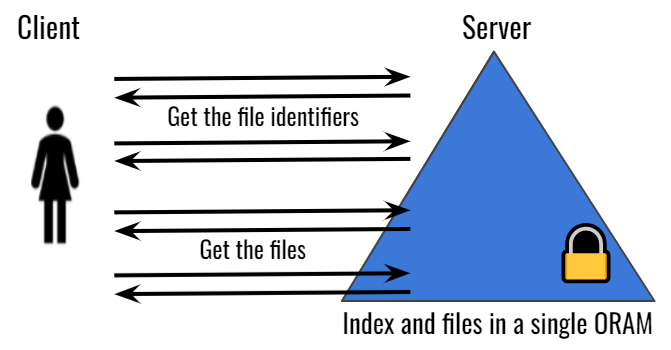
\includegraphics[scale=.3]{pictures/borion.png}
\caption{\BigOrion search for a single keyword $w$}
\end{figure}
\BigOrion stores the inverted index and the files in a single OMAP\footnote{Specifically, it is an AVL tree based oblivious data structure.}. 
%
During the setup phase, the client initializes two empty OMAPs of size $N$: $O_b$ and $O_{del}$. 
%
$N$ is the upper bound of the total number of entries $O_b$, and $O_{del}$ will ever store. 
%
Each key of $O_b$ maps to a value of $B$ bytes.
%
Apart from the index and the files, $O_b$ also stores \emph{file-count}\footnote{file-count: number of files that contain the keyword} of each keyword.
%
For a keyword $w$, its \emph{file-count} is denoted as $fcnt_w$.
%




Each key of $O_{del}$ maps a keyword-file identifier pair, $\pair{w}{id}$, to the number of files that contains $w$ at the time of inserting file $id$. Storing this information in $O_{del}$ makes it easier to substitute the last index entry (of $w$) with the deleted index entry (of $w$) in $O_{b}$. This \emph{substitution} makes subsequent searches for $w$ efficient.



\noindent\textbf{Insert.} To insert a file $f$ with identifier $id_f$, the client first divides $f$ into a total of $\ceil{{\vol{f}}/{B}}$ blocks, each of size $B$. 
%
The last block is padded, if needed. 
%
The client then stores the file blocks in the same order as they appear in $f$ at keys $\pair{id_f}{1},\pair{id_f}{2}, \ldots \pair{id_f}{\ceil{\frac{\vol{f}}{B}}}$. 
%
Next, for each unique keyword, $w$, that $f$ contains, the client increases the value of  $fcnt_w$, indicating one more file contains $w$ now. The client updates the index by mapping key $\pair{w}{fcnt_w}$ to $id_f$.
%
The client also inserts a mapping from key $\pair{w}{id_f}$ to value $fcnt_w$ in $O_{del}$, indicating $id_f$ is the $fcnt_w$th file to contain $w$.



\noindent\textbf{Delete.} To delete a file, the client retrieves the file blocks to compute the unique keywords and then it deletes the file blocks from $O_b$.
%
Deletion of the index entries are performed exactly like the deletes in \Orion \cite{Mitra}, i.e. for a particular keyword $w$ the deleted index entry is \emph{substituted} with the last index entry. 
%
This process guarantees that during a search query for $w$, the file identifiers are always retrieved by $\vol{\DB{w}}$ ORAM accesses.
%
In \BigOrion this number is even lesser, we will see why. 
%
Unlike \Orion, the last index entry is deleted after the substitution in \Bigorion.







\noindent\textbf{Optimized search.} During a standard \BigOrion search, the client first retrieves all the file identifiers from the index; and then it retrieves all the file blocks for each file identifier. Apart from the \emph{substitution} during deletes, \BigOrion implements three more optimization mechanisms to make the searches efficient: 
\begin{enumerate}
    \item  \emph{packing} the file identifiers,
    \item storing \emph{block-count}\footnote{block-count: number of blocks required to store the file} of each file, and
    \item utilizing ORAM \emph{batch-search}es
\end{enumerate}


The size of each file identifier is $\gamma$ bytes, which is much smaller than $B$. Thus $\frac{B}{\gamma}$ file identifiers are \emph{packed} together and stored in one block of $O_b$. This reduces the number of ORAM accesses to fetch $\vol{\DB{w}}$ file identifiers to $\ceil{\frac{\vol{\DB{w}}}{B}\gamma}$ from $\vol{\DB{w}}$.
%, unlike \Orion \cite{Mitra}.

The rounds of interaction with the server during searches can be reduced by making use of the \emph{batch-search}es of Path-ORAM. A batch-search does not break obliviousness if every access in the batch is for a different entry in the ORAM. The client stores the \emph{block-count} of each file in $O_b$ to make use of the \emph{batch-search}es. During a search for keyword $w$, the client retrieves  $fcnt_w$ and \emph{block-count} values of each $f\in \DB{w}$ from $O_b$ to execute OMAP reads in batches. For instance if 
\emph{file-count} of keyword $w$ is $n$ then the client can search for keys $\pair{w}{1},\pair{w}{2},\ldots \pair{w}{\ceil{\frac{n}{B}\gamma}}$ in a batch and retrieve all the file identifiers $id_1,id_2,...id_n$, with $O(\log N)$ rounds of communication instead of $O(\frac{n}{B}\gamma\log N)$ rounds of communication with the server. Similarly, if \emph{block-count} of file $id$ is $b$, then the client can search for keys $\pair{id}{1},\pair{id}{2},\ldots \pair{id}{b}$ in a batch to retrieve the whole file with $O(\log N)$ rounds of communication instead of $O(b\log N)$. The client can even batch search index and file blocks together since \BigOrion stores them in the same OMAP. 

\noindent\textbf{Client storage.} $O_b$ and $O_{del}$ are stored at the server. Each OMAP needs a cache of size $O(\log^2 N)$ at the client, but they can be stored at the server and downloaded during every operation. The client needs to store the secret key $K$ and the addresses of the roots of the AVL trees. Thus the permanent client storage of \Bigorion is $O(1)$.



\noindent\textbf{Security analysis.}
Because of the use of oblivious maps, the sequence of memory addresses accessed during any two operations are indistinguishable to the server. Dummy accesses are used to hide the volume pattern related leakages. 
%Hiding volume pattern leakages in entirety is not possible unless worst case padding is used. Any padding lesser than worst case padding leaks some information to the server. 
During \emph{setup}, the sizes of $O_b$ and $O_{del}$ are revealed to the server: $\mathcal{L}^{Stup} = \{N\}$.


When keywords and file blocks of a file $f$ are inserted (or deleted), the server would not be able to correlate the corresponding memory accesses with memory accesses pertaining to older search queries, which makes \BigOrion \textbf{forward-private}. The number of fake accesses used to hide the keyword count of the file is $\ceil{\frac{f}{B}}B-\kw{f}$, because there can be at most $\ceil{\frac{f}{B}}B$ keywords in worst case. The block-count of the file is revealed during an update, which reveals the actual file size when it is multiple of $B$.
The type of the operation, $op=\{ins,del\}$, is also revealed as the server observes two different patterns of interleavings of accesses to $O_b$ and $O_{del}$ during $insert$ and $delete$. Thus leakage profile of update operations is: $\mathcal{L}^{Updt}(op,id,f) = \{op,\vol{f}\}$. 

\BigOrion is more secure than \textbf{BP-I}. Accesses to $O_b$ during a search seem to be at uniformly random locations to the server; i.e, the server would not be able to figure out when the index entries pertaining to the searched keyword and the files containing the keyword were inserted. The only information server would have is the total number of accesses to $O_b$ which reveals the total volume of data retrieved by the client. The server would not know individual file sizes or $a_w$. 

We define, total file size (rounded off to nearest block size), $\tvol{w}$, number of blocks required to store file identifiers, $\idvol{w}$, and the summation of the two, $\tvold{w}$, as follows:
\begin{align*}
   % tvol(w) &= \sum_{f \in \DB{w}} \mid \ceil{f/B}*B \mid \\
   \tvol{w} &= \sum_{f \in \DB{w}} \ceil{\frac{\vol{f}}{B}}B & 
   \idvol{w} &= \ceil{\frac{\vol{\DB{w}}}{B}\gamma}B \\
 &   & \tvold{w} & =  \tvol{w} + \idvol{w}
\end{align*} 
%\footnote{$tvol'(w) > TVol(w)$, as $TVol(w)$ is the actual total volume of files}
Fake accesses are added at the end of the search operation to make the total number of accesses to $O_b$ equal to nearest power of $x$ (for $x\geq 2$). The total number of accesses to $O_b$ during a search including the dummy accesses is denoted as $\tvoldx{w}$, i.e. $\tvoldx{w}=x^n$ such that $x^{n-1} <  \tvold{w} \leq x^n$, (for $n\geq 1$). The leakage profile during search is: $\mathcal{L}_x^{Srch}(w) = \{\tvoldx{w}\}$.

As the server would not be able to figure out the individual file sizes, the \textsf{Subgraph}$^{vol}$ attack from \cite{Volat}, that depends on individual file sizes, is not possible on \Bigorion. \tred{Moreover, the client fetches whole paths from the Path-ORAM. Hence, individual file identifiers would not be revealed, which makes \textsf{Subgraph}$^{ID}$ attack from \cite{Volat} on \BigOrion impossible.} 
Due to the fake accesses to $O_b$ at the end of search operation, the \textsf{VolAn} and \textsf{SelVolAn} attacks from \cite{Volat} on \BigOrion are difficult. The bigger the value of $x$ is, the weaker the \textsf{VolAn} and \textsf{SelVolAn} attacks would be. 

\noindent\textbf{Further Optimization.}
We optimize \BigOrion further by storing the file blocks and the index into two separate OMAPs, instead of a single OMAP. We call this optimized scheme \Orionsq. \tred{\Orionsq is faster than \BigOrion because the paths fetched during each oblivious access are now smaller.} \emph{Packing} of file identifiers is not required anymore as the block size of the index OMAP is $\gamma$. But, during search the number of accesses to the index is now revealed to the server. 
$$\mathcal{L}^{Srch}_x=\{\DB{w},\tvolx{w}\}$$



\begin{lemma} \label{lemma:tvidv}
$ \tvol{w} \geq \idvol{w}$
\end{lemma}

\begin{proof}
Let us proof this with induction over $\vol{\DB{w}}$.\\
\textbf{Base case $\mathbf{\vol{\DB{w}}=1}$:}
This means only one file contains $w$. So,
$\idvol{w}=B$ and because every file has at least one block we can write $\tvol{w} \geq B$. Because $B \geq B$ we have  
$\tvol{w} \geq \idvol{w}$.\\
\textbf{Inductive hypothesis $\mathbf{\vol{\DB{w}}=n}$:} $n$ identifiers will require total of $\idvol{w} =\ceil{\frac{n}{B}\gamma}B$ blocks, and $n$ file will consist of at least $n$ blocks:, i.e. 
$\tvol{w} \geq nB$. Thus, from induction hypothesis( for $k=B/\gamma$), we have : 
\begin{equation}\label{eq:tvidv1}
nB \geq \ceil{\frac{n}{k}}B
\end{equation}
\textbf{Inductive Case $\mathbf{\vol{\DB{w}}=n+1}$:} $\idvol{w} =\ceil{\frac{n+1}{k}}B$, and $\tvol{w} = (n+1)B$, need to prove $(n+1)B \geq \ceil{\frac{n+1}{k}}B$
\begin{align*}
    (n+1)B & = nB +B \\ \intertext{from equation \ref{eq:tvidv1}}
        nB +B   & \geq \ceil{\frac{n}{k}}B +B \\
           & = \ceil{\frac{n}{k}}B +\ceil{\frac{k}{k}}B \\
           & \geq \ceil{\frac{n+k}{k}}B\\
           & \geq \ceil{\frac{n+1}{k}}B
\end{align*}
\end{proof}

\begin{lemma}
$ \idvol{w} = \alpha \tvol{w}$ for some $\alpha \leq 1$
\end{lemma}
\begin{proof}
From Lemma \ref{lemma:tvidv} we have $\idvol{w} \leq \tvol{w}$, i.e. either
$$\idvol{w} = \tvol{w}$$ in which case $\idvol{w} = \al \tvol{w}$ for $\al = 1$, or,
$$\idvol{w} < \tvol{w}$$
in which case $\idvol{w} = \al \tvol{w}$ for $\al < 1$. Hence, it is always the case that $\al \leq 1$
\end{proof}
\begin{figure}
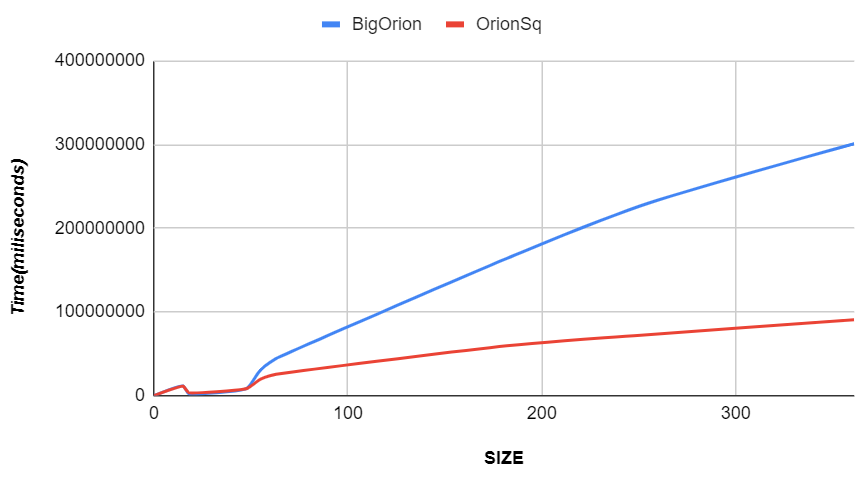
\includegraphics[scale=.3]{pictures/svsressize1.png}
\caption{search time (in miliseconds) vs variable result size for |D| = 361, |KW| = 1266 }
\end{figure}


\priyanka{position map in storage - not clear}
\appendix


\begin{acks}
Acknowledgement
\end{acks}


\bibliographystyle{ACM-Reference-Format}
\bibliography{citations}



\section{\BigOrion}
\BigOrion stores the \textbf{index} and the \textbf{files} in a single oblivious map, $O_{b}$. Each key of $O_{b}$ maps to $B$ bytes of data; the data can either be file identifiers (for the \textbf{index}), or file content (for the \textbf{files}). Each file identifier is of $\gamma$ bytes, and each keyword in a file can be of at most $\beta$ bytes (and of 1 byte minimum). $B$, $\gamma$, and $\beta$ are publicly known parameters. In our \BigOrion implementation $B$ is always bigger than and divisible by $\gamma$. 

\BigOrion maintains another oblivious map, $O_{del}$. The main purpose of having $O_{del}$ is to enable readjustments of elements of $O_{b}$ pertaining to a keyword, during a \emph{delete}; to make subsequent searches for the keyword efficient (details below). Each key of $O_{del}$ maps to a 4 byte integer.
For each keyword $w$, $O_{del}$ stores the number of files that contains $w$ at the time of inserting file $id$ at key $\pair{w}{id}$. In other words, if $\pair{w}{id}$ is mapped to $\kappa$, then file $id$ is the $\kappa$th file to contain $w$. This counter is denoted as $fcnt_w^{id}$.

$O_{b}$ stores two kinds of $(key,value)$ mappings. One for the files and the other for the index:
\begin{enumerate}
\item at key $\pair{w}{0}$, it stores the total number of files in the database that contains $w$, i.e. the \emph{file count} for $w$. This counter is denoted as $fcnt_w$.  When a new file containing $w$ is inserted, $fcnt_w$ is increased by one (and decremented when the file is deleted). 
    \item a file $f$, with identifier $id$, is divided into $n (=\ceil{\vol{f}/B})$ blocks ($b_1,...,b_n$), each of size $B$ bytes. The last block is padded if it is lesser than $B$ bytes. Block $b_i$ ($1 \leq i \leq n$) is stored at key $\pair{id}{i}$.
    
    \item for each unique keyword $w$ in $f$, the file identifier $id$ is stored (appended) at key $ \pair{w}{pk}$. We call $pk$ the \emph{pack number} for $id$ and is calculated as $\ceil{(fcnt_w/B)*\gamma}$. At most $B/\gamma$ (as $\gamma \mid B$) file identifiers can be packed together at one entry of $O_{b}$. We call this process $packing$ of file identifiers. Identifier $id$ is mapped at key $\pair{w}{pk}$ if file $id$ contains $w$ and the corresponding $fnct_w^{id}$ is in the following range:
    $$\frac{(pk-1)*B}{\gamma}+1 \leq fcnt_w^{id} \leq \frac{pk*B}{\gamma}$$ 
\end{enumerate}


\noindent\textbf{Setup.}
In the setup phase (see Algorithm \ref{alg:bosetup}) the client generates a secret key $K$  (line \ref{bosetalgo:keygen}) to encrypt and decrypt the values stored to and fetched from the server. The client sets up the two empty oblivious maps, $O_{b}$ and $O_{del}$, of sizes $N$ and $N'$ respectively, and stores them in the server as the encrypted database, $EDB$ (lines \ref{bosetalgo:omapsrc} -  \ref{bosetalgo:EDB}).  The client maintains a local state $\sigma$ (line \ref{bosetalgo:sigma}), which stores information (e.g. the roots of $O_{b}$ and $O_{del}$) to access the $EDB$.


\begin{algorithm}
\caption{\BigOrion $(K,\sigma; EDB) \leftarrow$ Setup($\lambda$,N)}\label{alg:bosetup}
\begin{algorithmic}[1]
\State $K \gets Gen(1^{\lambda})$ \label{bosetalgo:keygen}\yannis{We need to expand this.}
\State $(\sigma_{src}; O_{b}) \leftarrow \textsc{OmapSetup}(K,N)$ \label{bosetalgo:omapsrc} \yannis{I will find a better name}
\State $(\sigma_{del}; O_{del}) \leftarrow \textsc{OmapSetup}(K,N)$ \label{bosetalgo:omapdel} 
\State $EDB \gets (O_{b}, O_{del})$\label{bosetalgo:EDB}

\State Let $\sigma$ to be ($\sigma_{src},\sigma_{del}$) \label{bosetalgo:sigma}
\State \textbf{return} $(K,\sigma; EDB)$
\end{algorithmic}
\label{Algo:BigorionSetup}
\end{algorithm}


\begin{algorithm}
\caption{\BigOrion $(K,\sigma; EDB) \leftrightarrow$ $Insert(K, id, f, \sigma; EDB)$}\label{alg:boi}
\begin{algorithmic}[1]
%\If{$op$ = $insert$}
\State$\{b_1,...,b_n\} \gets$ Divide $f$ into blocks of size $B$, pad $b_n$ if needed  \label{boinsalgo:blocks}
\For{$i=1$ to $n$}
  \State $\tblue{O_{b}.Insert(\pair{id}{i},b_i)}$
 \EndFor \label{boinsalgo:insblocks}
  \State $\tblue{O_{b}.Insert(\pair{id}{(n+1)},NULL)}$ \label{boinsalgo:nullblock}
 \State Get all unique keywords of $f$ in set $KW$ 
 %\State Initialize empty map $U$
 \For{each $w \in KW$} \label{boinsalgo:forloopstart}
    \State $fcnt_w \gets \tblue{O_{b}.Find(\pair{w}{0})}$ \label{boinsalgo:getfcnt}
    \State $fcnt_w \gets (fcnt_w=NULL)?1:fcnt_w$\texttt{++}\label{boinsalgo:fcntincr}
    
    \State $\tblue{O_{b}.Insert(\pair{w}{0},fcnt_w)}$\label{boinsalgo:setfcnt} \label{boinsalgo:fcntupdt}
    \State $\tblue{O_{del}.Insert(\pair{w}{id},fcnt_w)}$\label{boinsalgo:fcntidupdt}
   \State \textcolor{red}{$pk \gets \ceil{(fcnt_w/B)*\gamma})$}\label{boinsalgo:getpk} \Comment{get the $pack$ number}
    %Compute  the place to insert $id$ for $w$ using $(U[w])$}
    \State $\textcolor{red}{ids \gets O_{b}.Find(\pair{w}{pk})}$ \Comment{$ids$ can be NULL}\label{boinsalgo:findidblock}
 \State \textcolor{red}{Append $id$ to $ids$ } \label{boinsalgo:appendid}
   \State $\tblue{O_{b}.Insert(\pair{w}{pk},ids)}$\label{boinsalgo:updtidblock}
\EndFor \label{boinsalgo:forloopend}
%\State $\textcolor{purple}{O_{b}.Finalize(2*\mu_f)}$
\State \tblue{1 access to $O_{del}$ and 4 accesses to $O_{b}$, in loop, for $(nB-\vol{KW})$ times} \label{boinsalgo:fake}
\State $EDB \gets (O_{b},O_{del})$ 
\end{algorithmic}
\label{Algo:BigorionInsert}
\end{algorithm}

\noindent\textbf{Insert.} To insert a file (see Algorithm \ref{alg:boi}) $f$ with identifier $id$, the client first inserts the blocks of $f$ one by one (lines \ref{boinsalgo:blocks} - \ref{boinsalgo:insblocks}). The client stores a $NULL$ value as the last file block (line \ref{boinsalgo:nullblock}), so that during a \emph{search} it will know when to stop fetching file blocks. Next, for each unique keyword $w$ of file $f$, the client obliviously accesses $O_{del}$ thrice and $O_{b}$ twice (line \ref{boinsalgo:forloopstart} - \ref{boinsalgo:forloopend}). The client retrieves the file count $fcnt_w$ from $O_{del}$ at key $\pair{w}{0}$ (line \ref{boinsalgo:getfcnt}), sets its value to 1 if $w$ is inserted for the first time, otherwise increases its value by 1 (line \ref{boinsalgo:fcntincr}). The client updates the value at key $\pair{w}{0}$ with the increased value of $fcnt_w$ (line \ref{boinsalgo:setfcnt}). This indicates one more file contains $w$ now. The client also inserts a mapping from key $\pair{w}{id}$ to $fcnt_w$ (line \ref{boinsalgo:fcntidupdt}) in $O_{del}$, indicating $id$ is the $fcnt_w$th file to contain $w$. Next, the client computes $pk$, the \emph{pack number} for $w$ (line \ref{boinsalgo:getpk}), to retrieve the \emph{pack} of identifiers from key $\pair{w}{pk}$ of $O_{b}$ (line \ref{boinsalgo:findidblock} ). It appends $id$ to the existing \emph{pack} of identifiers (or inserts $id$ if the \emph{pack} was empty) (line \ref{boinsalgo:appendid}) and maps the updated block back at key $\pair{w}{pk}$ (line \ref{boinsalgo:updtidblock}). A file of size $n$ blocks can have at most $nB$ keywords (considering every keyword to be of 1 byte in worst case). Hence, the client simulates dummy accesses for $nB-\vol{KW}$ keywords at the end (line \ref{boinsalgo:fake} ). 




\noindent\textbf{Delete.}
During a \emph{delete} of a file $id$ (see Algorithm \ref{alg:bodel}), the client first deletes the file blocks from $O_{b}$ (lines \ref{bodelalg:repeat} - \ref{bodelalg:until}). Next, for each unique keyword $w$ of file $id$, the client retrieves $fcnt_w^{id}$ and $fcnt_w$ from $O_{del}$ from keys $\pair{w}{id}$ and $\pair{w}{0}$  respectively (lines \ref{bodelalg:getfcntidw}, \ref{bodelalg:getfcntw}); the client removes the entry at $\pair{w}{id}$ (line \ref{bodelalg:removeidw}) and decreases the value of \emph{file count} (line \ref{bodelalg:setfcntw}), indicating that one less file contains $w$ now. The client then retrieves and removes the identifier $id_{last}$, that was inserted last, from the last \emph{pack} of identifiers for keyword $w$ (lines \ref{bodelalg:getlastids} - \ref{bodelalg:setlastidsendif}), from $O_{b}$. The client substitutes $id$ with $id_{last}$ at key $\pair{w}{pk_{del}}$ (lines \ref{bodelalg:getpkdel} - \ref{bodelalg:updtdelids}) in $O_{b}$, $pk_{del}$ being the \emph{pack number} for $id$. Substituting $id$ with $id_{last}$ guarantees that during a \emph{search} of $w$ the $fcnt_w$ file identifiers are retrieved from the keys $\pair{w}{1}\ldots \pair{w}{\ceil{\frac{fcnt_w}{B}*\gamma}}$ with exact ${\ceil{\frac{fcnt_w}{B}*\gamma}}$ accesses to $O_{b}$. The client also substitutes the value at key $\pair{w}{id_{last}}$ with $fcnt_w^{id}$ in $O_{del}$, to use this information during future deletes (line \ref{bodelalg:updtfcntidw}). Finally, the client performs fake accesses for the worst case number of keywords (line \ref{bodelalg:fakeaccs}).

\begin{algorithm}
\caption{\BigOrion$(K,\sigma;EDB) \leftrightarrow Delete(K,id,\bot,\sigma;EDB)$}\label{alg:bodel}
\begin{algorithmic}[1]
 \State $Content=``"$ \Comment{Empty string}
 %\State $\textcolor{blue}{block \gets O_{b}.Find(\pair{id}{1})}$
 \State $blocknum \gets 0$ 
 \Repeat \label{bodelalg:repeat}
 %\While{{$block != NULL$}}
    \State $block \gets\tblue{ (O_{b}.Find(\pair{id}{\texttt{++}blocknum}})$
     \State Append $block$ to $Content$  \label{bodelalg:appendcont}
    \State $\tblue{O_{b}.Remove(\pair{id}{blocknum})}$  \label{bodelalg:removeblk}
\Until{$block = NULL$} \label{bodelalg:until}
%\EndWhile{$block != NULL$}
\State \emph{unpad} $Content$ and get all unique keywords in set $KW$ \label{bodelalg:uniqkey}
\For{each $w \in KW$}  \label{bodelalg:foreachkey}
\State $fcnt_{w}^{id} \gets \tblue{ O_{del}.Find(\pair{w}{id})}$  \label{bodelalg:getfcntidw}
\State $fcnt_{w} \gets \tblue{O_{b}.Find(\pair{w}{0})}$ \label{bodelalg:getfcntw}
\State $\tblue{O_{del}.Remove(\pair{w}{id})}$ \label{bodelalg:removeidw}
 \State $\tblue{O_{b}.Insert(\pair{w}{0},fcnt_{w}-1)}$ \label{bodelalg:setfcntw}
\State \textcolor{red}{$pk_{last} \gets \ceil{(fcnt_w/B)*\gamma}$ }\label{bodelalg:getpklast}
%Compute the place of last pack of ids from $fcnt_w$}
\State $lastids \gets \tblue{ O_{b}.Find(\pair{w}{pk_{last}})}$\label{bodelalg:getlastids}
\State \textcolor{red}{$id_{last} \gets$ retrieve the last $identifier$ from $lastids$ }\label{bodelalg:getlastid}
\State \textcolor{red}{$lastids \gets$ remove $id_{last}$ from $lastids$}\label{bodelalg:updtlastids}
\If{\textcolor{red}{$lastids = NULL$}}
 \State $\textcolor{blue}{O_{b}.Remove(\pair{w}{pk_{last}})}$\label{bodelalg:remlastids}
 \Else \State \textcolor{red}{{$O_{b}.Insert(\pair{w}{pk_{last}},lastids)$}}\label{bodelalg:setlastids}
 \EndIf \label{bodelalg:setlastidsendif}
  \If{$fcnt_{w}^{id} \neq fcnt_{w}$} \Comment{i.e. $id$ is not the last entry}
  \State \textcolor{red}{$pk_{del} \gets \ceil{(fcnt_w^{id}/B)*\gamma} $} \label{bodelalg:getpkdel}
  %compute the place of $id$ from $fdel_w$}
  \State \textcolor{red}{$delids \gets O_{b}.Find(\pair{w}{pk_{del}})$}\label{bodelalg:getdelids}
  \State \textcolor{red}{replace $id$ with $id_{last}$ in $delids$}\label{bodelalg:insdelids}
   \State $\tblue{O_{b}.Insert(\pair{w}{pk_{del}}),delids)}$\label{bodelalg:updtdelids}
    \State $\tblue{O_{del}.Insert(\pair{w}{id_{last}},fcnt_{w}^{id})}$\label{bodelalg:updtfcntidw}
  \EndIf
\EndFor
\State \tblue{3 accesses to $O_{del}$ and 5 accesses to $O_{b}$ in loop, for $((blocknum-1)*B) - \vol{KW}$ dummy keywords}\label{bodelalg:fakeaccs}
\State $EDB \gets (O_{b},O_{del})$
\end{algorithmic}
\label{Algo:BigorionDelete}
\end{algorithm}



\noindent\textbf{Search.} The \emph{search} algorithm (Algorithm \ref{alg:bos}) for a keyword $w$ is very simple. The client first retrieves the file count, $fcnt_w$ (line \ref{bosrchalg:getfcntw}), to compute the number of \emph{packs} for $w$. Next, the client retrieves all the file identifiers (lines \ref{bosrchalg:forid} - \ref{bosrchalg:endforid}) from $O_{b}$. Finally, the client fetches all the file blocks (line \ref{bosrchalg:forfile} - \ref{bosrchalg:endforfile}), and then adds some fake accesses at the end (to the nearest power of $x$) to hide the actual number of accesses to $O_{b}$ (line \ref{bosrchalg:fake}). 



\begin{algorithm}
\caption{\BigOrion $\DB{w} \leftrightarrow$ Search($K$,$w$,$\sigma$; EDB)}\label{alg:bos}
\begin{algorithmic}[1]
\State {$fcnt_{w} \gets \tblue{O_{b}.Find(\pair{w}{0})}$} \label{bosrchalg:getfcntw}
\State Initialize empty set $ID$
 \For{ $i=$ 1 to $\ceil{(fcnt_{w}/B)*\gamma}$} \label{bosrchalg:forid} \Comment{$\gamma$ is size of file identifiers} 
   \State $idblock \gets \tblue{O_{b}.Find(\pair{w}{i})}$
   \State $ID = ID \cup\{$ retrieve all identifiers from $idblock$ as a set $\}$
\EndFor \label{bosrchalg:endforid}
%\State add $(\vol{DB} - \vol{\DB{w}})$ dummy accesses to $O_{b}$  
 \State Initialize an empty map $Files$ 
\For{each $id \in ID$} \label{bosrchalg:forfile}
%\State $\textcolor{blue}{block \gets  O_{b}.Find(\pair{id}{1})}$
%\State $i \gets 1$
%  \While{$block~ != ~NULL$}  
\State $blk \gets 0$
\Repeat
\State $block \gets\tblue{ O_{b}.Find(\pair{id}{\texttt{++}blk})}$
     \State Append $block$ to $Files[id]$ 
  \Until{$block~ = ~NULL$}
  \EndFor \label{bosrchalg:endforfile}
  %\State $x^n-blk$ accesses to $O_{b}$ \Comment{$x^{(n-1)} <  blk \leq x^n$}
  \State \tblue{add dummy accesses to $O_{b}$, total of $x^n$ accesses} \label{bosrchalg:fake}

\State $\DB{w} \gets Files$
\end{algorithmic}
\label{Algo:BigorionSearch}
\end{algorithm}





\noindent\textbf{Optimization.}
Although we showed the standard version of the \emph{search} algorithm in Algorithm \ref{alg:bos}, in our real implementation we make use of the OMAP \emph{batch-search} which makes the searches even more efficient. For this, during insert, instead of making last file block $NULL$, we store total number of blocks (\textbf{block-size}) of the file at key $\pair{id}{0}$, in $O_{b}$. Then, for a search of a keyword $w$, we do the following accesses to $O_{b}$:
\begin{enumerate}
    \item fetch the first \emph{pack} of the file identifiers from key  $\pair{w}{1}$ 
    \item batch search the rest of the \emph{pack}s of file identifiers from keys $\pair{w}{2}$ $\ldots$ $\pair{w}{pk}$ (where, $pk=\ceil{fcnt_w/B}*\gamma$) and the block-size of first $B/\gamma$ files, from keys $\pair{id_1}{0}$$\ldots$$\pair{id_{B/\gamma}}{0}$, plus some fake accesses to make the size of this batch $b=x^n$ (nearest power of $x$)
    \item at this point the client has all the file identifiers, so all the block-sizes can be retrieved in the next batch-search along with some file blocks
    \item perform a series of batch searches to retrieve rest of the file blocks, making each batch size to be $b$
\end{enumerate}


%\noindent\textbf{Time Complexity.} based on the optimizations mentioned above LATER
%\noindent\textbf{Storage.} LATER
\section{\Orionsq}

\begin{algorithm}
\caption{\Orionsq $(K,\sigma; EDB) \leftarrow$ Setup($\lambda$,N)}\label{alg:osqsetup}
\begin{algorithmic}[1]
\State $K \gets Gen(1^{\lambda})$ \label{osetalgo:keygen}\yannis{We need to expand this.}
\State $(\sigma_{f}; OMAP_{f}) \leftarrow \textsc{OmapSetup}(K,N)$
\State $(\sigma_{src}; O_{b}) \leftarrow \textsc{OmapSetup}(K)$ \label{osetalgo:omapsrc} \yannis{I will find a better name}
\State $(\sigma_{del}; O_{del}) \leftarrow \textsc{OmapSetup}(K)$ \label{osetalgo:omapdel}
\State $EDB \gets (OMAP_{f}, O_{b}, O_{del})$ \label{bosetalgo:edb}
\State Let $\sigma$ to be ($\sigma_{f}, \sigma_{src},\sigma_{del}$) \label{osetalgo:sigma}
\State \textbf{return} $(K,\sigma; EDB)$
\end{algorithmic}
\label{Algo:orionsqSetup}
\end{algorithm}








\begin{algorithm}
\caption{\Orionsq $ (K,\sigma';EDB')\leftrightarrow Insert(K,\pair{id}{f},\sigma; EDB)$}\label{orionspins}
\begin{algorithmic}[1]
\State$\{b_1,...,b_n\} \gets$ Divide $f$ into blocks of size $B$, pad $b_n$ if needed  \label{oinsalgo:blocks}
\For{$i=1$ to $n$}
  \State $\textcolor{blue}{OMAP_{f}.Insert(\pair{id}{i},b_i)}$
 \EndFor \label{oinsalgo:insblocks}
  \State $\tblue{OMAP_{f}.Insert(\pair{id}{(n+1)},NULL)}$ \label{oinsalgo:nullblock}
  %\State Fake accesses to $OMAP_f$ $(x^m-(n-1))$ times
 \State Get all unique keywords of $f$ in set $KW$ 
 %\State Initialize empty map $U$
 \For{each $w \in KW$} \label{oinsalgo:forloopstart}
    \State $fcnt_w \gets \tblue{O_{del}.Find(\pair{w}{0})}$ \label{oinsalgo:getfcnt}
    \State $fcnt_w \gets (fcnt_w=NULL)?1:fcnt_w$\texttt{++} \label{oinsalgo:fcntinc}
    \State $\tblue{O_{del}.Insert(\pair{w}{0},fcnt_w)}$\label{oinsalgo:setfcnt} \label{oinsalgo:fcntupdt}
    \State $\tblue{O_{del}.Insert(\pair{w}{id},fcnt_w)}$\label{oinsalgo:fcntidupdt}
   \State $\tblue{O_{b}.Insert(\pair{w}{fcnt_w},id)}$\label{oinsalgo:updtidblock}
\EndFor \label{oinsalgo:forloopend}
%\State $\textcolor{purple}{O_{b}.Finalize(2*\mu_f)}$
\State \tblue{3 accesses to $O_{del}$ and 1 access to $O_{b}$, in loop, for $(nB-\vol{KW})$ times} \label{oinsalgo:fake}
\State $EDB \gets (OMAP_{f},O_{b},O_{del})$ 
\end{algorithmic}
\label{Algo:orionsqUpdate}
\end{algorithm}


\begin{algorithm}
\caption{\Orionsq $(K,\sigma;EDB) \leftrightarrow Delete(K,\pair{id}{\bot},\sigma; EDB)$}\label{orionplus:delete}
\begin{algorithmic}[1]
\State $file=``"$ \Comment{Empty string}
 %\State $\textcolor{blue}{block \gets O_{b}.Find(\pair{id}{1})}$
 \State $blocknum \gets 0$ 
 \Repeat \label{odelalg:repeat}
    \State $block \gets\tblue{ (OMAP_{f}.Find(\pair{id}{\texttt{++}blocknum}})$
     \State Append $block$ to $file$  \label{odelalg:appendcont}
    \State $\tblue{OMAP_{f}.Remove(\pair{id}{blocknum})}$  \label{odelalg:removeblk}
\Until{$block = NULL$} \label{odelalg:until}
%\EndWhile{$block != NULL$}
\State Get all unique keywords of $file$ in set $KW$ \label{odelalg:uniqkey}
\For{each $w \in KW$}  \label{odelalg:foreachkey}
\State $fcnt_{w}^{id} \gets \tblue{ O_{del}.Find(\pair{w}{id})}$  \label{odelalg:getfcntidw}
\State $fcnt_{w} \gets\tblue{ O_{del}.Find(\pair{w}{0})}$ \label{odelalg:getfcntw}
\State $\tblue{O_{del}.Remove(\pair{w}{id})}$ \label{odelalg:removeidw}
 \State $\tblue{O_{del}.Insert(\pair{w}{0},fcnt_{w}-1)}$ \label{odelalg:setfcntw}
\State $id_{last} \gets \tblue{ O_{b}.Find(\pair{w}{fcnt_w})}$\label{odelalg:getlastids}
\State $\tblue{O_{b}.Remove(\pair{w}{fcnt_w})}$\label{odelalg:remlastids}
 
\If{$fcnt_{w}^{id} \neq fcnt_{w}$} \Comment{i.e. $id$ is not the last entry}
 
\State $\tblue{O_{b}.Insert(\pair{w}{fcnt_w^{id}}),id_{last})}$\label{odelalg:updtdelids}
  \State $\tblue{O_{del}.Insert(\pair{w}{id_{last}},fcnt_{w}^{id})}$\label{odelalg:updtfcntidw}
  \EndIf
\EndFor
\State \tblue{5 accesses to $O_{del}$ and 3 accesses to $O_{b}$ in loop for $((blocknum-1)*B) - \vol{KW}$ dummy keywords} \label{odelalg:fake}
\State $EDB \gets (OMAP_f,O_{b},O_{del})$
\end{algorithmic}
\label{Algo:orion2pUpdate}
\end{algorithm}



\begin{algorithm}
\caption{\Orionsq $\DB{w} \leftrightarrow Search(K,w,\sigma; EDB)$}\label{alg:orionsqs}
\begin{algorithmic}[1]
\State Initialize empty set $R$
\State $fcnt_{w} \gets \tblue{O_{del}.Find(\pair{w}{0})}$
 \For{ $i$= 1 to $fcnt_{w}$}
   \State $id \gets \tblue{O_{b}.Find(\pair{w}{i})}$
   \State $R \gets R \cup \{id\}$
\EndFor
 \State{\tblue{$(y^m-fcnt_w)$ fake accesses to $O_{b}$}} \Comment{nearest power of $y$} \label{alg:osqsearchbkt}
 \State Initialize empty map $File$ 
\For{each $id \in R$}
\State $blk \gets 1$
  \Repeat
      \State $block \gets \tblue{OMAP_{f}.Find(\pair{id}{blk\texttt{++}})}$
     \State append $block$ to $File[id]$ 
    %\Comment{appends the block content}
 \Until{$block = NULL$}
\EndFor
\State {\tblue{Fake accesses to $OMAP_{f}$, total of $x^n$ accesses}}
\State $\DB{w} \gets Files$
\end{algorithmic}
\label{Algo:orion2pSearch}
\end{algorithm}


\subsection{Security Analysis of \Orionsq}
$$\mathcal{L}^{Stup} = \{N\}$$
$$\mathcal{L}^{Updt}(op,id,f) = \{op,\vol{\ceil{f/B}*B}\}$$
$$\mathcal{L}_x^{Srch}(w) = \{bvol(w),tvol_x(w)\}$$
$bvol(w)$ is the total number of accesses to $O_{b}$, in worst case it is equal to $\DB{w}$ (see line \ref{alg:osqsearchbkt} in Algorithm \ref{alg:orionsqs})

\section{\Orionp}


\begin{algorithm}
\caption{\Orionp $(K,\sigma;EDB)\leftarrow Setup(\lambda,N)$}\label{alg:orionpsetup}
\begin{algorithmic}[1]
\State $K \gets Gen(1^{\lambda})$
\State Initialize empty dictionary $DictF$ for files
\State $(\sigma_{f};OMAP_{f})\gets \textsc{OmapSetup}(K,N)$ 
\State $(\sigma_{src};O_{b})\gets \textsc{OmapSetup}(K,N)$ 
\State $(\sigma_{del},O_{del}) \gets \textsc{OmapSetup}(K,N)$
\State Let $\sigma$ to be ($\sigma_{f}, \sigma_{src},\sigma_{del}$) \label{opsetalgo:sigma}
\State $EDB \gets (DictF, OMAP_f, O_{b}, O_{del})$
\State Send $EDB$ to Server
\State \textbf{return} $(K,\sigma; EDB)$
\end{algorithmic}
\end{algorithm}
\label{Algo:Orion+Setup}






\begin{algorithm}
\caption{\Orionp $(K,\sigma; EDB)\leftarrow Insert(K,\sigma,(id,f);EDB)$}\label{alg:orionpinsert}
\begin{algorithmic}[1]
\State pad $f$ to size $nB$ \Comment{multiple of $B$}  \label{opinsalgo:pad}
\State $addr \gets G_K(id,1||0)$
  \State $DictF[addr] \gets f \oplus G_K(id,1||1)$
  \label{opinsalgo:insblocks}
  \State \tblue{$OMAP_{ac}.Insert(id,1)$}
\State Get all unique keywords of $f$ in set $KW$ 
 %\State Initialize empty map $U$
 \For{each $w \in KW$} \label{opinsalgo:forloopstart}
    \State $fcnt_w \gets\tblue{ O_{del}.Find(\pair{w}{0})}$ \label{opinsalgo:getfcnt}
    \State $fcnt_w\gets(fcnt_w=NULL)?1:fcnt_w$\texttt{++} \label{opinsalgo:fcntinc}
    \State $\tblue{O_{del}.Insert(\pair{w}{0},fcnt_w)}$\label{opinsalgo:setfcnt} \label{opinsalgo:fcntupdt}
    \State $\tblue{O_{del}.Insert(\pair{w}{id},fcnt_w)}$\label{opinsalgo:fcntidupdt}
   \State $\tblue{O_{b}.Insert(\pair{w}{fcnt_w},id)}$\label{opinsalgo:updtidblock}
\EndFor \label{opinsalgo:forloopend}
%\State $\textcolor{purple}{O_{b}.Finalize(2*\mu_f)}$
\State \tblue{3 accesses to $O_{del}$ and 1 access to $O_{b}$, in loop, for $(nB-\vol{KW})$ times} \label{opinsalgo:fake}
\State $EDB \gets (DictF,OMAP_{f},O_{b},O_{del})$
\end{algorithmic}
\end{algorithm}
\label{Algo:Orion+insert}


\begin{algorithm}
\caption{\Orionp $(K,\sigma; EDB)\leftarrow Delete(K,\sigma,(id,\bot);EDB)$}\label{alg:orionpdelete}
\begin{algorithmic}[1]
 \State \tblue{$ac \gets OMAP_f.Find(id)$}
\State $addr \gets G_K(id,ac||0)$
  \State $f \gets DictF[addr] \oplus G_K(id,ac||1)$
  \label{opinsalgo:delblocks}
\State $unpad$ $f$ and get all unique keywords in set $KW$ 
 %\State Initialize empty map $U$
 \For{each $w\in$  $KW$}
 \State $fcnt_{w}^{id} \gets \tblue{ O_{del}.Find(\pair{w}{id})}$  \label{opdelalg:getfcntidw}
\State $fcnt_{w} \gets  \tblue{O_{del}.Find(\pair{w}{0})}$ \label{opdelalg:getfcntw}
\State $ \tblue{O_{del}.Remove(\pair{w}{id})}$ \label{opdelalg:removeidw}
 \State $ \tblue{O_{del}.Insert(\pair{w}{0},fcnt_{w}-1)}$ \label{opdelalg:setfcntw}
\State $ id_{last} \gets \tblue{ O_{b}.Find(\pair{w}{fcnt_w})}$\label{opdelalg:getlastids}

 \State $ \tblue{O_{b}.Remove(\pair{w}{fcnt_w})}$\label{opdelalg:remlastids}
 
  \If{$fcnt_{w}^{id} \neq fcnt_{w}$} \Comment{i.e. $id$ is not the last entry}
 
    \State $ \tblue{O_{b}.Insert(\pair{w}{fcnt_w^{id}}),id_{last})}$\label{opdelalg:updtdelids}
  \State $ \tblue{O_{del}.Insert(\pair{w}{id_{last}},fcnt_{w}^{id})}$\label{opdelalg:updtfcntidw}
  \EndIf
  \EndFor
%\State $\textcolor{purple}{O_{b}.Finalize(2*\mu_f)}$
\State \tblue{accesses to $O_{del}$ and $O_{b}$, in loop, for $(\vol{f}-\vol{KW})$ times} \label{opdelalgo:fake}
\State $EDB \gets (DictF,OMAP_{f},O_{b},O_{del})$
\end{algorithmic}
\end{algorithm}
\label{Algo:Orion+delete}



\begin{algorithm}
\caption{\Orionp $\DB{w}\leftarrow Search(K,\sigma,w;EDB)$}\label{alg:orionpsearch}
\begin{algorithmic}[1]
\State Initialize empty set $R$
\State $fcnt_{w} \gets \tblue{O_{del}.Find(\pair{w}{0})}$
 \For{ $i$= 1 to $fcnt_{w}$}
   \State $id \gets \tblue{O_{b}.Find(\pair{w}{i})}$
   \State $R \gets R \cup \{id\}$
\EndFor
 \State{\tblue{$(y^m-fcnt_w)$ fake accesses to $O_{b}$}} \Comment{nearest power of $y$}
 \State add $(y^m-fcnt_w)$ fake $id$s to $R$
 \State Initialize empty map $Files$
\For{$i$ = 1 to $|R|$}
\State $ac \gets \tblue{OMAP_f.Find(R[i])}$
\State $f \gets DictF[G_K(R[i],ac||0)] \oplus (G_K(R[i],ac||1))$
\State $Files \gets Files \cup \{f\}$
\State $\texttt{++}ac$
\State \tblue{$OMAP_f.Insert(R[i],ac)$}
\State $addr \gets G_K(R[i],ac||0)$
\State $DictF[addr] \gets f \oplus G_K(R[i],ac||1)$
  \EndFor
%\Statex \textbf{At Client:}
\State $\DB{w} \gets Files$
 
\end{algorithmic}
\end{algorithm}
\label{Algo:Orion+Search}

\subsection{Security analysis of \Orionp}
Other than $ap$ and $sp$ \Orionp has the following leakages:
$$\mathcal{L}^{Stup} = \{N\}$$
$$\mathcal{L}^{Updt}(op,id,f) = \{op,\vol{f}\}$$
$$\mathcal{L}^{Srch}(w) = \{bvol(w),vol(w)\}$$
$bvol(w)$ is the total number of accesses to $O_{b}$, in worst case it is equal to $\DB{w}$;
$vol(w)$ leaks $tvol(w)$ as well

\section{\Mitrap}



\begin{algorithm}
\caption{\Mitrap$(K,\sigma;EDB)$ $\leftarrow$ Setup($\lambda$,DB)}\label{mitap:setup}
\begin{algorithmic}[1]
\State $K \gets Gen(1^{\lambda})$
%\State Generate map $G : W \rightarrow Int$ \Comment{maps $kw$ to its bucket frequency}
%\State $DB' \gets Fake\_Doc\_Gen(DB,G)$
\State $(\sigma_{ac},OMAP_{ac}) \gets \textsc{OmapSetup}(K,N)$\Comment{stores  $accsCnt$}
\State $(\sigma_{kw};OMAP_{kw})\gets \textsc{OmapSetup}(K,N'
)$\Comment{stores $fileCnt$, $srcCnt$}
\State Initialize $DictW$ and $DictF$
\State $\sigma \gets (\sigma_{ac},\sigma_{kw})$
\State $EDB \gets  (DictF,OMAP_{ac},DictW,OMAP_{kw})$
\State Send $EDB$ to Server
\end{algorithmic}
\end{algorithm}
\label{Algo:Mitra+Setup}


\begin{algorithm}[tbh]
\caption{\Mitrap $(K,\sigma';EDB')$ $\leftrightarrow$ $Insert(K,op,\pair{id}{f},\sigma;EDB)$}\label{alg:orionplusInsert}
\begin{algorithmic}[1]
\State pad $f$ to be of size $mB$ \Comment{multiple of $B$}
\State $add_f \gets G_K(id,1||0)$
\State $DictF[add_f] \gets f \oplus G_K(id,1||1)$
\State \tblue{$OMAP_{ac}.Insert(id,1)$}
\State Get all unique keyword of $f$ in set $KW$
\For{$all ~ w \in KW$}
\State $\tblue{\pair{fc}{sc} \gets OMAP_{kw}(w)}$
\State $add_w \gets G_K(w,fc||sc||0)$
\State $DictW[add_w] \gets id||ins \oplus G_K(w,fc||sc||1)$
\State \tblue{$OMAP.Insert(w,\pair{fc+1}{sc})$}
\EndFor
\end{algorithmic}
\end{algorithm}
\label{Algo:Mitra+Update}



\begin{algorithm}[tbh]
\caption{\Mitrap $(K,\sigma';EDB')$ $\leftrightarrow$ $Delete(K,op,\pair{id}{\bot},\sigma;EDB)$}\label{mitrap:delete}
\begin{algorithmic}[1]
\State \tblue{$ac \gets OMAP_{ac}.Find(id)$}
\State $add_f \gets G_K(id,ac||0)$
\State $f \gets DictF[add_f] \oplus G_K(id,ac||1)$
\State $unpad$ $f$ and get unique keywords in set $KW$
\For{$all ~ w \in KW$}
\State $\tblue{\pair{fc}{sc} \gets OMAP_{kw}(w)}$
\State $add_w \gets G_K(w,fc+1||sc||0)$
\State $DictW[add_w] \gets id||del \oplus G_K(w,fc||sc||1)$
\State \tblue{$OMAP.Insert(w,\pair{fc+1}{sc})$}
\EndFor
\end{algorithmic}
\end{algorithm}
\label{Algo:Mitra+Delete}



\begin{algorithm}[H]
\caption{\Mitrap $\DB{w}$ $\leftrightarrow$ Search($K$,$w$,$\sigma$;$EDB$)}\label{mitra:search}
\begin{algorithmic}[1]
%\Statex \textbf{At Client:}
\State $T = \{ \}$
\State $\pair{fc}{sc} \gets \tblue{OMAP_{kw}.Find(w)}$
\State Initialize set $ID$
\For{$i = 1$ to $fc$} 
  \State $add_w \gets \{G_K(w,i||sc||0)\}$
  \State $id||op \gets DictW[add_w] \oplus  \{G_K(w,i||sc||1)\}$
  \If{$op=ins$} add $id$ to $ID$
  \EndIf
  \State $add_w \gets \{G_K(w,i||sc+1||0)\}$
  \State $DictW[add_w] \gets id||op \oplus G_K(w,i||sc+1||1)$
  \State \tblue{$OMAP_{kw}.Insert(w,\pair{fc}{sc+1})$}
\EndFor
\For{each $id \in ID$}
\State $ac \gets \tblue{OMAP.Find(id)}$
\State $add_f \gets G_K(id,ac||0)$
\State $f \gets DictF[add_f] \oplus G_K(id,ac||1) $
\State add $f$ to $\DB{w}$
\State $\tblue{OMAP.Insert(id,ac+1)}$
\EndFor
\end{algorithmic}
\end{algorithm}
\label{Algo:Mitra+Search}


\subsection{Security analysis of \Mitrap}
Other than $ap$ and $sp$ \Mitrap has following leakages:
$$\mathcal{L}^{Stup} = \{N,N'\}$$
$$\mathcal{L}^{Updt}(op,id,f) = \{op,\vol{\ceil{f/B}*B},kc\}$$
$$\mathcal{L}^{Srch}(w) = 
\{a_w,rlp,vol(w)\}$$
$vol(w)$ leaks $tvol(w)$
\section{Proofs}

\subsection{Part One}


\subsection{Part Two}


\section{Online Resources}


\end{document}
\endinput
